\documentclass[twoside]{book}

% Packages required by doxygen
\usepackage{fixltx2e}
\usepackage{calc}
\usepackage{doxygen}
\usepackage[export]{adjustbox} % also loads graphicx
\usepackage{graphicx}
\usepackage[utf8]{inputenc}
\usepackage{makeidx}
\usepackage{multicol}
\usepackage{multirow}
\PassOptionsToPackage{warn}{textcomp}
\usepackage{textcomp}
\usepackage[nointegrals]{wasysym}
\usepackage[table]{xcolor}

% Font selection
\usepackage[T1]{fontenc}
\usepackage[scaled=.90]{helvet}
\usepackage{courier}
\usepackage{amssymb}
\usepackage{sectsty}
\renewcommand{\familydefault}{\sfdefault}
\allsectionsfont{%
  \fontseries{bc}\selectfont%
  \color{darkgray}%
}
\renewcommand{\DoxyLabelFont}{%
  \fontseries{bc}\selectfont%
  \color{darkgray}%
}
\newcommand{\+}{\discretionary{\mbox{\scriptsize$\hookleftarrow$}}{}{}}

% Page & text layout
\usepackage{geometry}
\geometry{%
  a4paper,%
  top=2.5cm,%
  bottom=2.5cm,%
  left=2.5cm,%
  right=2.5cm%
}
\tolerance=750
\hfuzz=15pt
\hbadness=750
\setlength{\emergencystretch}{15pt}
\setlength{\parindent}{0cm}
\setlength{\parskip}{3ex plus 2ex minus 2ex}
\makeatletter
\renewcommand{\paragraph}{%
  \@startsection{paragraph}{4}{0ex}{-1.0ex}{1.0ex}{%
    \normalfont\normalsize\bfseries\SS@parafont%
  }%
}
\renewcommand{\subparagraph}{%
  \@startsection{subparagraph}{5}{0ex}{-1.0ex}{1.0ex}{%
    \normalfont\normalsize\bfseries\SS@subparafont%
  }%
}
\makeatother

% Headers & footers
\usepackage{fancyhdr}
\pagestyle{fancyplain}
\fancyhead[LE]{\fancyplain{}{\bfseries\thepage}}
\fancyhead[CE]{\fancyplain{}{}}
\fancyhead[RE]{\fancyplain{}{\bfseries\leftmark}}
\fancyhead[LO]{\fancyplain{}{\bfseries\rightmark}}
\fancyhead[CO]{\fancyplain{}{}}
\fancyhead[RO]{\fancyplain{}{\bfseries\thepage}}
\fancyfoot[LE]{\fancyplain{}{}}
\fancyfoot[CE]{\fancyplain{}{}}
\fancyfoot[RE]{\fancyplain{}{\bfseries\scriptsize Generated by Doxygen }}
\fancyfoot[LO]{\fancyplain{}{\bfseries\scriptsize Generated by Doxygen }}
\fancyfoot[CO]{\fancyplain{}{}}
\fancyfoot[RO]{\fancyplain{}{}}
\renewcommand{\footrulewidth}{0.4pt}
\renewcommand{\chaptermark}[1]{%
  \markboth{#1}{}%
}
\renewcommand{\sectionmark}[1]{%
  \markright{\thesection\ #1}%
}

% Indices & bibliography
\usepackage{natbib}
\usepackage[titles]{tocloft}
\setcounter{tocdepth}{3}
\setcounter{secnumdepth}{5}
\makeindex

% Hyperlinks (required, but should be loaded last)
\usepackage{ifpdf}
\ifpdf
  \usepackage[pdftex,pagebackref=true]{hyperref}
\else
  \usepackage[ps2pdf,pagebackref=true]{hyperref}
\fi
\hypersetup{%
  colorlinks=true,%
  linkcolor=blue,%
  citecolor=blue,%
  unicode%
}

% Custom commands
\newcommand{\clearemptydoublepage}{%
  \newpage{\pagestyle{empty}\cleardoublepage}%
}

\usepackage{caption}
\captionsetup{labelsep=space,justification=centering,font={bf},singlelinecheck=off,skip=4pt,position=top}

%===== C O N T E N T S =====

\begin{document}

% Titlepage & ToC
\hypersetup{pageanchor=false,
             bookmarksnumbered=true,
             pdfencoding=unicode
            }
\pagenumbering{alph}
\begin{titlepage}
\vspace*{7cm}
\begin{center}%
{\Large vector.\+h }\\
\vspace*{1cm}
{\large Generated by Doxygen 1.8.13}\\
\end{center}
\end{titlepage}
\clearemptydoublepage
\pagenumbering{roman}
\tableofcontents
\clearemptydoublepage
\pagenumbering{arabic}
\hypersetup{pageanchor=true}

%--- Begin generated contents ---
\chapter{vector.\+h}
\label{md_README}
\Hypertarget{md_README}
A toy single-\/header C library for vector math.

\subsection*{Usage}

After cloning the repository, simply run {\ttfamily make} to compile the test suite. 
\chapter{Data Structure Index}
\section{Data Structures}
Here are the data structures with brief descriptions\+:\begin{DoxyCompactList}
\item\contentsline{section}{\hyperlink{structVec2}{Vec2} }{\pageref{structVec2}}{}
\item\contentsline{section}{\hyperlink{structVec3}{Vec3} }{\pageref{structVec3}}{}
\end{DoxyCompactList}

\chapter{File Index}
\section{File List}
Here is a list of all files with brief descriptions\+:\begin{DoxyCompactList}
\item\contentsline{section}{\hyperlink{tests_8c}{tests.\+c} }{\pageref{tests_8c}}{}
\item\contentsline{section}{\hyperlink{vector_8h}{vector.\+h} }{\pageref{vector_8h}}{}
\end{DoxyCompactList}

\chapter{Data Structure Documentation}
\hypertarget{structVec2}{}\section{Vec2 Struct Reference}
\label{structVec2}\index{Vec2@{Vec2}}


{\ttfamily \#include $<$vector.\+h$>$}

\subsection*{Data Fields}
\begin{DoxyCompactItemize}
\item 
int \hyperlink{structVec2_ae76e144847d9ef65bd288df4dc83f8a3}{x}
\item 
int \hyperlink{structVec2_af8c49fd3e96353c332024c4c48057539}{y}
\end{DoxyCompactItemize}


\subsection{Detailed Description}
Simple structure for a 2D vector 
\begin{DoxyParams}[1]{Parameters}
\mbox{\tt in}  & {\em x} & coordinate of the vector \\
\hline
\mbox{\tt in}  & {\em y} & coordinate of the vector \\
\hline
\end{DoxyParams}


\subsection{Field Documentation}
\mbox{\Hypertarget{structVec2_ae76e144847d9ef65bd288df4dc83f8a3}\label{structVec2_ae76e144847d9ef65bd288df4dc83f8a3}} 
\index{Vec2@{Vec2}!x@{x}}
\index{x@{x}!Vec2@{Vec2}}
\subsubsection{\texorpdfstring{x}{x}}
{\footnotesize\ttfamily int Vec2\+::x}

\mbox{\Hypertarget{structVec2_af8c49fd3e96353c332024c4c48057539}\label{structVec2_af8c49fd3e96353c332024c4c48057539}} 
\index{Vec2@{Vec2}!y@{y}}
\index{y@{y}!Vec2@{Vec2}}
\subsubsection{\texorpdfstring{y}{y}}
{\footnotesize\ttfamily int Vec2\+::y}



The documentation for this struct was generated from the following file\+:\begin{DoxyCompactItemize}
\item 
\hyperlink{vector_8h}{vector.\+h}\end{DoxyCompactItemize}

\hypertarget{structVec3}{}\section{Vec3 Struct Reference}
\label{structVec3}\index{Vec3@{Vec3}}


{\ttfamily \#include $<$vector.\+h$>$}

\subsection*{Data Fields}
\begin{DoxyCompactItemize}
\item 
int \hyperlink{structVec3_a47ccb74f80c697cf605475aa53e541ea}{x}
\item 
int \hyperlink{structVec3_a836a1434ee2b949cd24d356afcaf56b4}{y}
\item 
int \hyperlink{structVec3_ae81b73bbda5bfa26b648a44158bf6d36}{z}
\end{DoxyCompactItemize}


\subsection{Detailed Description}
Simple structure for a 3D vector 
\begin{DoxyParams}[1]{Parameters}
\mbox{\tt in}  & {\em x} & coordinate of the vector \\
\hline
\mbox{\tt in}  & {\em y} & coordinate of the vector \\
\hline
\mbox{\tt in}  & {\em z} & coordinate of the vector \\
\hline
\end{DoxyParams}


\subsection{Field Documentation}
\mbox{\Hypertarget{structVec3_a47ccb74f80c697cf605475aa53e541ea}\label{structVec3_a47ccb74f80c697cf605475aa53e541ea}} 
\index{Vec3@{Vec3}!x@{x}}
\index{x@{x}!Vec3@{Vec3}}
\subsubsection{\texorpdfstring{x}{x}}
{\footnotesize\ttfamily int Vec3\+::x}

\mbox{\Hypertarget{structVec3_a836a1434ee2b949cd24d356afcaf56b4}\label{structVec3_a836a1434ee2b949cd24d356afcaf56b4}} 
\index{Vec3@{Vec3}!y@{y}}
\index{y@{y}!Vec3@{Vec3}}
\subsubsection{\texorpdfstring{y}{y}}
{\footnotesize\ttfamily int Vec3\+::y}

\mbox{\Hypertarget{structVec3_ae81b73bbda5bfa26b648a44158bf6d36}\label{structVec3_ae81b73bbda5bfa26b648a44158bf6d36}} 
\index{Vec3@{Vec3}!z@{z}}
\index{z@{z}!Vec3@{Vec3}}
\subsubsection{\texorpdfstring{z}{z}}
{\footnotesize\ttfamily int Vec3\+::z}



The documentation for this struct was generated from the following file\+:\begin{DoxyCompactItemize}
\item 
\hyperlink{vector_8h}{vector.\+h}\end{DoxyCompactItemize}

\chapter{File Documentation}
\hypertarget{README_8md}{}\section{R\+E\+A\+D\+M\+E.\+md File Reference}
\label{README_8md}\index{R\+E\+A\+D\+M\+E.\+md@{R\+E\+A\+D\+M\+E.\+md}}

\hypertarget{tests_8c}{}\section{tests.\+c File Reference}
\label{tests_8c}\index{tests.\+c@{tests.\+c}}
{\ttfamily \#include $<$stdio.\+h$>$}\newline
{\ttfamily \#include \char`\"{}C\+Unit/\+C\+Unit.\+h\char`\"{}}\newline
{\ttfamily \#include \char`\"{}C\+Unit/\+Basic.\+h\char`\"{}}\newline
{\ttfamily \#include \char`\"{}vector.\+h\char`\"{}}\newline
Include dependency graph for tests.\+c\+:
\nopagebreak
\begin{figure}[H]
\begin{center}
\leavevmode
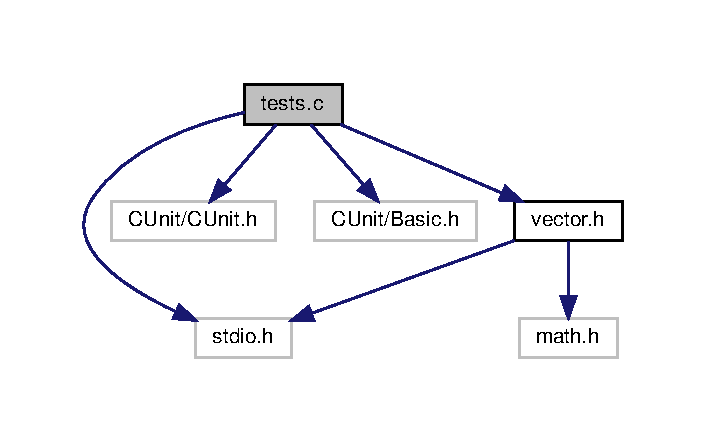
\includegraphics[width=339pt]{tests_8c__incl}
\end{center}
\end{figure}
\subsection*{Functions}
\begin{DoxyCompactItemize}
\item 
int \hyperlink{tests_8c_a11244ab0910e8dbcdf132f10630dea91}{init\+\_\+suite} (void)
\item 
int \hyperlink{tests_8c_a1277ae7ecbaaad1479cfac38aaa7891d}{clean\+\_\+suite} (void)
\item 
void \hyperlink{tests_8c_afd00fbf4b32f8c7e6a3aa7b3ab33e755}{vec2\+\_\+test\+\_\+points} (void)
\item 
void \hyperlink{tests_8c_aa2ccb77fde4fb830c2e1d8f7c2f99472}{vec2\+\_\+test\+\_\+swap} (void)
\item 
void \hyperlink{tests_8c_a0a453bb5e5bc877d66512fc0bfd9cb0f}{vec2\+\_\+test\+\_\+distance1} (void)
\item 
void \hyperlink{tests_8c_a4e7d2916cad0c54b60dce3b095f7ba3b}{vec2\+\_\+test\+\_\+distance2} (void)
\item 
void \hyperlink{tests_8c_acde402c8317799b3b49ef554d48b08fb}{vec2\+\_\+test\+\_\+distance3} (void)
\item 
int \hyperlink{tests_8c_a840291bc02cba5474a4cb46a9b9566fe}{main} (void)
\end{DoxyCompactItemize}


\subsection{Function Documentation}
\mbox{\Hypertarget{tests_8c_a1277ae7ecbaaad1479cfac38aaa7891d}\label{tests_8c_a1277ae7ecbaaad1479cfac38aaa7891d}} 
\index{tests.\+c@{tests.\+c}!clean\+\_\+suite@{clean\+\_\+suite}}
\index{clean\+\_\+suite@{clean\+\_\+suite}!tests.\+c@{tests.\+c}}
\subsubsection{\texorpdfstring{clean\+\_\+suite()}{clean\_suite()}}
{\footnotesize\ttfamily int clean\+\_\+suite (\begin{DoxyParamCaption}\item[{void}]{ }\end{DoxyParamCaption})}

\mbox{\Hypertarget{tests_8c_a11244ab0910e8dbcdf132f10630dea91}\label{tests_8c_a11244ab0910e8dbcdf132f10630dea91}} 
\index{tests.\+c@{tests.\+c}!init\+\_\+suite@{init\+\_\+suite}}
\index{init\+\_\+suite@{init\+\_\+suite}!tests.\+c@{tests.\+c}}
\subsubsection{\texorpdfstring{init\+\_\+suite()}{init\_suite()}}
{\footnotesize\ttfamily int init\+\_\+suite (\begin{DoxyParamCaption}\item[{void}]{ }\end{DoxyParamCaption})}

\mbox{\Hypertarget{tests_8c_a840291bc02cba5474a4cb46a9b9566fe}\label{tests_8c_a840291bc02cba5474a4cb46a9b9566fe}} 
\index{tests.\+c@{tests.\+c}!main@{main}}
\index{main@{main}!tests.\+c@{tests.\+c}}
\subsubsection{\texorpdfstring{main()}{main()}}
{\footnotesize\ttfamily int main (\begin{DoxyParamCaption}\item[{void}]{ }\end{DoxyParamCaption})}

\mbox{\Hypertarget{tests_8c_a0a453bb5e5bc877d66512fc0bfd9cb0f}\label{tests_8c_a0a453bb5e5bc877d66512fc0bfd9cb0f}} 
\index{tests.\+c@{tests.\+c}!vec2\+\_\+test\+\_\+distance1@{vec2\+\_\+test\+\_\+distance1}}
\index{vec2\+\_\+test\+\_\+distance1@{vec2\+\_\+test\+\_\+distance1}!tests.\+c@{tests.\+c}}
\subsubsection{\texorpdfstring{vec2\+\_\+test\+\_\+distance1()}{vec2\_test\_distance1()}}
{\footnotesize\ttfamily void vec2\+\_\+test\+\_\+distance1 (\begin{DoxyParamCaption}\item[{void}]{ }\end{DoxyParamCaption})}

\mbox{\Hypertarget{tests_8c_a4e7d2916cad0c54b60dce3b095f7ba3b}\label{tests_8c_a4e7d2916cad0c54b60dce3b095f7ba3b}} 
\index{tests.\+c@{tests.\+c}!vec2\+\_\+test\+\_\+distance2@{vec2\+\_\+test\+\_\+distance2}}
\index{vec2\+\_\+test\+\_\+distance2@{vec2\+\_\+test\+\_\+distance2}!tests.\+c@{tests.\+c}}
\subsubsection{\texorpdfstring{vec2\+\_\+test\+\_\+distance2()}{vec2\_test\_distance2()}}
{\footnotesize\ttfamily void vec2\+\_\+test\+\_\+distance2 (\begin{DoxyParamCaption}\item[{void}]{ }\end{DoxyParamCaption})}

\mbox{\Hypertarget{tests_8c_acde402c8317799b3b49ef554d48b08fb}\label{tests_8c_acde402c8317799b3b49ef554d48b08fb}} 
\index{tests.\+c@{tests.\+c}!vec2\+\_\+test\+\_\+distance3@{vec2\+\_\+test\+\_\+distance3}}
\index{vec2\+\_\+test\+\_\+distance3@{vec2\+\_\+test\+\_\+distance3}!tests.\+c@{tests.\+c}}
\subsubsection{\texorpdfstring{vec2\+\_\+test\+\_\+distance3()}{vec2\_test\_distance3()}}
{\footnotesize\ttfamily void vec2\+\_\+test\+\_\+distance3 (\begin{DoxyParamCaption}\item[{void}]{ }\end{DoxyParamCaption})}

\mbox{\Hypertarget{tests_8c_afd00fbf4b32f8c7e6a3aa7b3ab33e755}\label{tests_8c_afd00fbf4b32f8c7e6a3aa7b3ab33e755}} 
\index{tests.\+c@{tests.\+c}!vec2\+\_\+test\+\_\+points@{vec2\+\_\+test\+\_\+points}}
\index{vec2\+\_\+test\+\_\+points@{vec2\+\_\+test\+\_\+points}!tests.\+c@{tests.\+c}}
\subsubsection{\texorpdfstring{vec2\+\_\+test\+\_\+points()}{vec2\_test\_points()}}
{\footnotesize\ttfamily void vec2\+\_\+test\+\_\+points (\begin{DoxyParamCaption}\item[{void}]{ }\end{DoxyParamCaption})}

\mbox{\Hypertarget{tests_8c_aa2ccb77fde4fb830c2e1d8f7c2f99472}\label{tests_8c_aa2ccb77fde4fb830c2e1d8f7c2f99472}} 
\index{tests.\+c@{tests.\+c}!vec2\+\_\+test\+\_\+swap@{vec2\+\_\+test\+\_\+swap}}
\index{vec2\+\_\+test\+\_\+swap@{vec2\+\_\+test\+\_\+swap}!tests.\+c@{tests.\+c}}
\subsubsection{\texorpdfstring{vec2\+\_\+test\+\_\+swap()}{vec2\_test\_swap()}}
{\footnotesize\ttfamily void vec2\+\_\+test\+\_\+swap (\begin{DoxyParamCaption}\item[{void}]{ }\end{DoxyParamCaption})}


\hypertarget{vector_8h}{}\section{vector.\+h File Reference}
\label{vector_8h}\index{vector.\+h@{vector.\+h}}
{\ttfamily \#include $<$stdio.\+h$>$}\newline
{\ttfamily \#include $<$math.\+h$>$}\newline
Include dependency graph for vector.\+h\+:
\nopagebreak
\begin{figure}[H]
\begin{center}
\leavevmode
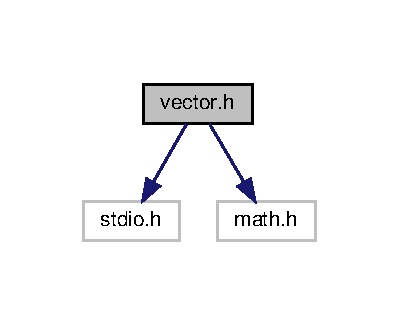
\includegraphics[width=192pt]{vector_8h__incl}
\end{center}
\end{figure}
This graph shows which files directly or indirectly include this file\+:
\nopagebreak
\begin{figure}[H]
\begin{center}
\leavevmode
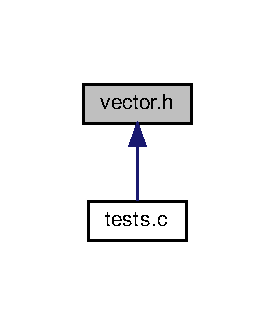
\includegraphics[width=132pt]{vector_8h__dep__incl}
\end{center}
\end{figure}
\subsection*{Data Structures}
\begin{DoxyCompactItemize}
\item 
struct \hyperlink{structVec2}{Vec2}
\item 
struct \hyperlink{structVec3}{Vec3}
\end{DoxyCompactItemize}
\subsection*{Typedefs}
\begin{DoxyCompactItemize}
\item 
typedef struct \hyperlink{structVec2}{Vec2} \hyperlink{vector_8h_a77ab0fbf6576acf1533cb7963655f77c}{Vec2}
\item 
typedef struct \hyperlink{structVec3}{Vec3} \hyperlink{vector_8h_accf408e3e7c8f0da0653692466f81a54}{Vec3}
\end{DoxyCompactItemize}
\subsection*{Functions}
\begin{DoxyCompactItemize}
\item 
void \hyperlink{vector_8h_a1e709f8cfb3f02dd75e205b0fb0e500e}{vec2\+\_\+swap\+\_\+points} (\hyperlink{structVec2}{Vec2} $\ast$vector)
\item 
int \hyperlink{vector_8h_a409d4800f56c90731ad9c70895b856ed}{vec2\+\_\+distance} (\hyperlink{structVec2}{Vec2} vector1, \hyperlink{structVec2}{Vec2} vector2)
\end{DoxyCompactItemize}


\subsection{Typedef Documentation}
\mbox{\Hypertarget{vector_8h_a77ab0fbf6576acf1533cb7963655f77c}\label{vector_8h_a77ab0fbf6576acf1533cb7963655f77c}} 
\index{vector.\+h@{vector.\+h}!Vec2@{Vec2}}
\index{Vec2@{Vec2}!vector.\+h@{vector.\+h}}
\subsubsection{\texorpdfstring{Vec2}{Vec2}}
{\footnotesize\ttfamily typedef struct \hyperlink{structVec2}{Vec2}  \hyperlink{structVec2}{Vec2}}

Simple structure for a 2D vector 
\begin{DoxyParams}[1]{Parameters}
\mbox{\tt in}  & {\em x} & coordinate of the vector \\
\hline
\mbox{\tt in}  & {\em y} & coordinate of the vector \\
\hline
\end{DoxyParams}
\mbox{\Hypertarget{vector_8h_accf408e3e7c8f0da0653692466f81a54}\label{vector_8h_accf408e3e7c8f0da0653692466f81a54}} 
\index{vector.\+h@{vector.\+h}!Vec3@{Vec3}}
\index{Vec3@{Vec3}!vector.\+h@{vector.\+h}}
\subsubsection{\texorpdfstring{Vec3}{Vec3}}
{\footnotesize\ttfamily typedef struct \hyperlink{structVec3}{Vec3}  \hyperlink{structVec3}{Vec3}}

Simple structure for a 3D vector 
\begin{DoxyParams}[1]{Parameters}
\mbox{\tt in}  & {\em x} & coordinate of the vector \\
\hline
\mbox{\tt in}  & {\em y} & coordinate of the vector \\
\hline
\mbox{\tt in}  & {\em z} & coordinate of the vector \\
\hline
\end{DoxyParams}


\subsection{Function Documentation}
\mbox{\Hypertarget{vector_8h_a409d4800f56c90731ad9c70895b856ed}\label{vector_8h_a409d4800f56c90731ad9c70895b856ed}} 
\index{vector.\+h@{vector.\+h}!vec2\+\_\+distance@{vec2\+\_\+distance}}
\index{vec2\+\_\+distance@{vec2\+\_\+distance}!vector.\+h@{vector.\+h}}
\subsubsection{\texorpdfstring{vec2\+\_\+distance()}{vec2\_distance()}}
{\footnotesize\ttfamily int vec2\+\_\+distance (\begin{DoxyParamCaption}\item[{\hyperlink{structVec2}{Vec2}}]{vector1,  }\item[{\hyperlink{structVec2}{Vec2}}]{vector2 }\end{DoxyParamCaption})}

Gets the dsiatance between two 2D vectors 
\begin{DoxyParams}[1]{Parameters}
\mbox{\tt in}  & {\em \hyperlink{structVec2}{Vec2}} & vector1 \\
\hline
\mbox{\tt in}  & {\em \hyperlink{structVec2}{Vec2}} & vector2 \\
\hline
\end{DoxyParams}
\begin{DoxyReturn}{Returns}
double The distance between them. 
\end{DoxyReturn}
\mbox{\Hypertarget{vector_8h_a1e709f8cfb3f02dd75e205b0fb0e500e}\label{vector_8h_a1e709f8cfb3f02dd75e205b0fb0e500e}} 
\index{vector.\+h@{vector.\+h}!vec2\+\_\+swap\+\_\+points@{vec2\+\_\+swap\+\_\+points}}
\index{vec2\+\_\+swap\+\_\+points@{vec2\+\_\+swap\+\_\+points}!vector.\+h@{vector.\+h}}
\subsubsection{\texorpdfstring{vec2\+\_\+swap\+\_\+points()}{vec2\_swap\_points()}}
{\footnotesize\ttfamily void vec2\+\_\+swap\+\_\+points (\begin{DoxyParamCaption}\item[{\hyperlink{structVec2}{Vec2} $\ast$}]{vector }\end{DoxyParamCaption})}

Swaps the x and y values of a Vector 
\begin{DoxyParams}[1]{Parameters}
\mbox{\tt in}  & {\em \hyperlink{structVec2}{Vec2}} & Pointer to a vector \\
\hline
\end{DoxyParams}
\begin{DoxyReturn}{Returns}
none 
\end{DoxyReturn}

%--- End generated contents ---

% Index
\backmatter
\newpage
\phantomsection
\clearemptydoublepage
\addcontentsline{toc}{chapter}{Index}
\printindex

\end{document}
